% BEGIN PREAMBEL
\documentclass[9pt]{beamer}
\usepackage[british]{babel}
\usepackage[latin1]{inputenc}
\usepackage{multimedia}
\usepackage{amsmath,amsfonts,amssymb}
\usepackage{upgreek}
\usepackage{pgfpages}
\usepackage[version=3]{mhchem}
\usepackage{lmodern}
\usepackage{graphicx}
\usepackage{multicol}
\usepackage{color}
\usepackage{xcolor,fontawesome}
\usepackage{wrapfig}
\usepackage{siunitx}
\usepackage{fontspec}
\usepackage{tikz}
\usepackage{textpos}
\newfontfamily\ubuntu{Ubuntu}
\newcommand{\as}{\\[14pt]}
\newcommand{\s}{\\[7pt]}
\newcommand{\is}{\\[2pt]}
\newcommand{\no}{\noindent}
\newcommand{\ka}{\hspace*{0.5cm}}
\newcommand{\ma}{\hspace*{1cm}}
\newcommand{\ga}{\hspace*{1.5cm}}
\newcommand{\li}{\left|}
\newcommand{\re}{\right|}
\newcommand{\const}{\text{const.}}
\newcommand{\z}{\text}
\newcommand{\terminal}[1]{\colorbox{black}{\textcolor{white}{{\fontfamily{phv}\selectfont \scriptsize{#1}}}}}
\newcommand{\plugin}[1]{\textit{\flq#1\frq}}
\definecolor{darkcerulean}{rgb}{0.03, 0.27, 0.49}
\newcommand{\ubu}[1]{{\color{darkcerulean}\footnotesize \ubuntu #1}}
\newcommand*\arc{{\fontfamily{pbk}\fontseries{db}\selectfont+}}
\usetheme{Boadilla}
\graphicspath{ {Pics/} }
\usecolortheme{beaver}
\useoutertheme{miniframes}
\beamertemplatenavigationsymbolsempty
\makeindex
\title[Analysis]{Discussion of the Pad Analysis}
\author[M. Reichmann]{Michael Reichmann}
\institute[\textbf{\textit{ETH}}\scalebox{.6}{\textit{Z\"{u}rich}}]{Swiss Federal Institute of Technology Zurich}
\AtBeginSection{\frame{\sectionpage}}
% END PREAMBEL
\begin{document}
% ============================
% BEGIN TITLE PAGE
% ============================
\usebackgroundtemplate{\tikz\node[opacity=0.2] {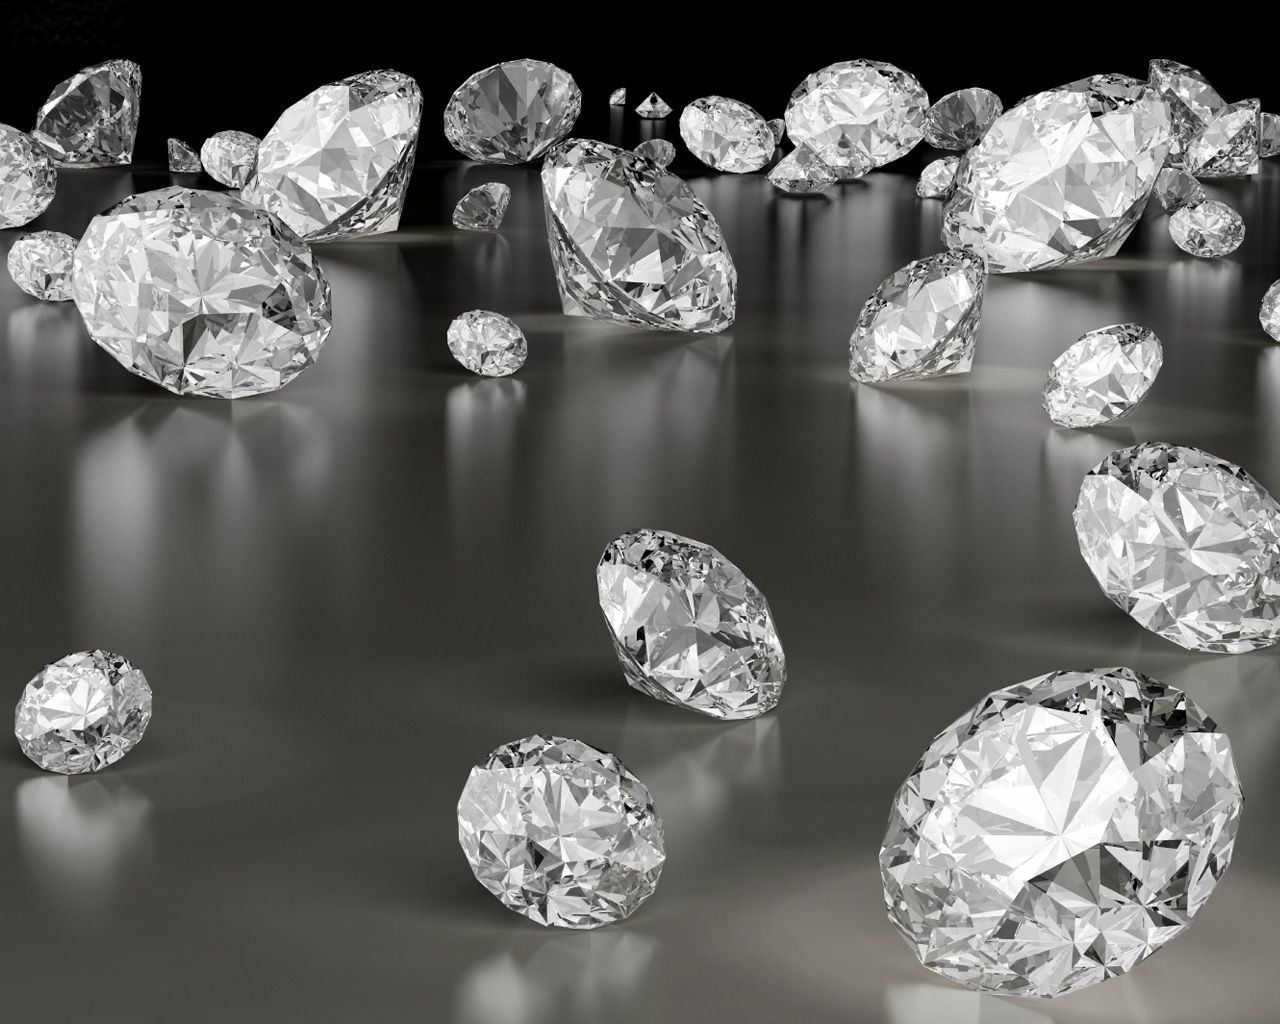
\includegraphics[height=\paperheight,width=\paperwidth]{bkg.jpg}};}
\begin{frame}
	\begin{center}
		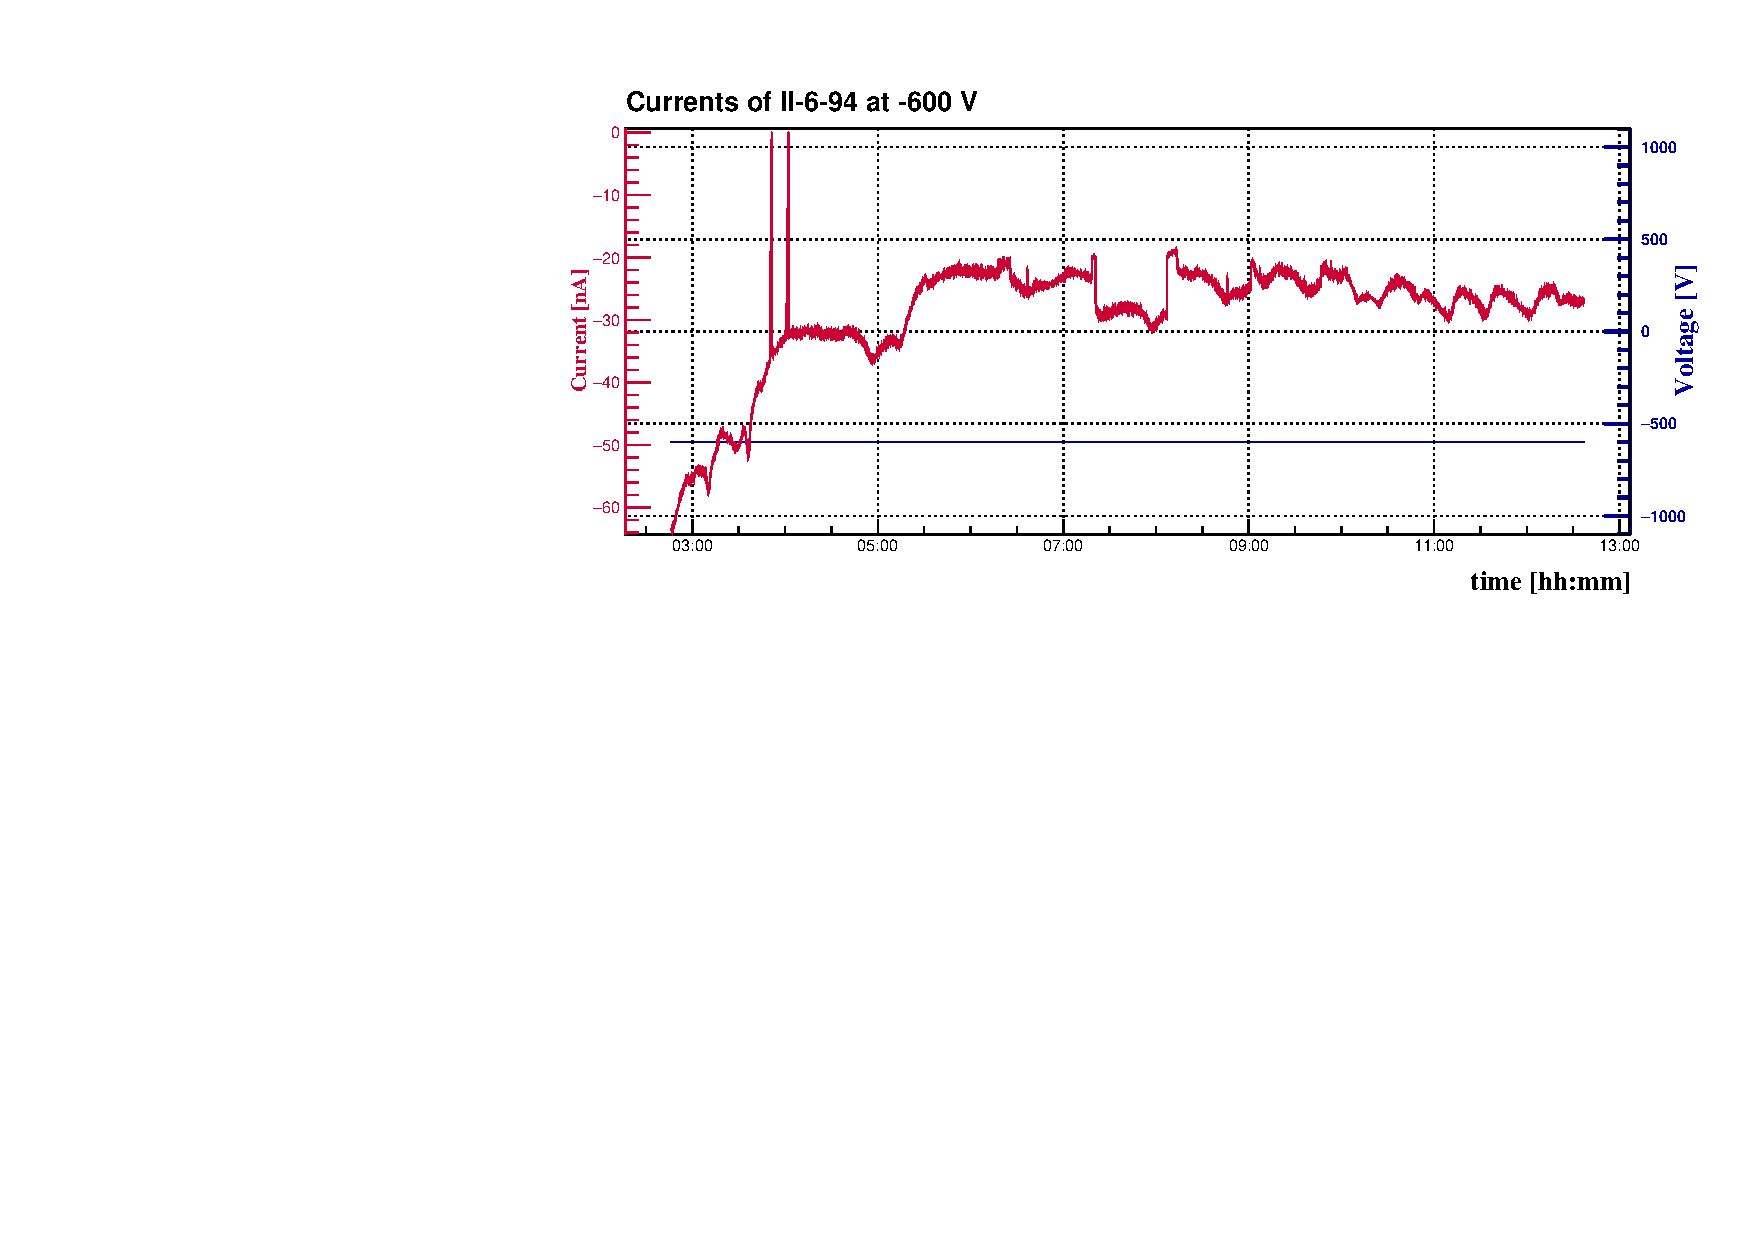
\includegraphics[angle=270, width=7cm]{II-6-94_-600}
	\end{center}
	\begin{alertblock}{
		\begin{center}
			\textbf{Measured currents of the diamonds for the next beam test}
		\end{center}}
		\vspace*{10pt}
		\begin{center}\small
		Speaker: Michael Reichmann
		\end{center}\normalsize
	\end{alertblock}
\end{frame}
\usebackgroundtemplate{}
% END
% ============================
% BEGIN TABLE OF CONTENTS
% ============================
\begin{frame}[allowframebreaks]
	\frametitle{Table of contents}
	\tableofcontents   % [pausesections]
\end{frame}
% END
% ====================================================================================
% BEGIN INTRO
% ====================================================================================
\section{Introduction}
% ============================
\begin{frame}
	\frametitle{Introduction}
	\begin{minipage}[c][.7\textheight]{6cm}
		\begin{itemize}
			\setlength{\itemsep}{\fill}
			\item interesting diamonds for the next beam test in August 2016
			\begin{itemize}
				\item II6-94
				\item II6-95
				\item II6-96
				\item II6-97
				\item II6-B2
			\end{itemize}
			\item check their current behaviour from the previous beam tests
		\end{itemize}
	\end{minipage}
\end{frame}
% ====================================================================================
% BEGIN II6-94
% ====================================================================================
\section{II6-94}
% ============================
\subsection{$-$\SI{600}{V}}
\begin{frame}
	\frametitle{$-$\SI{600}{V}}
	\vspace*{-15pt}
	\begin{center}
		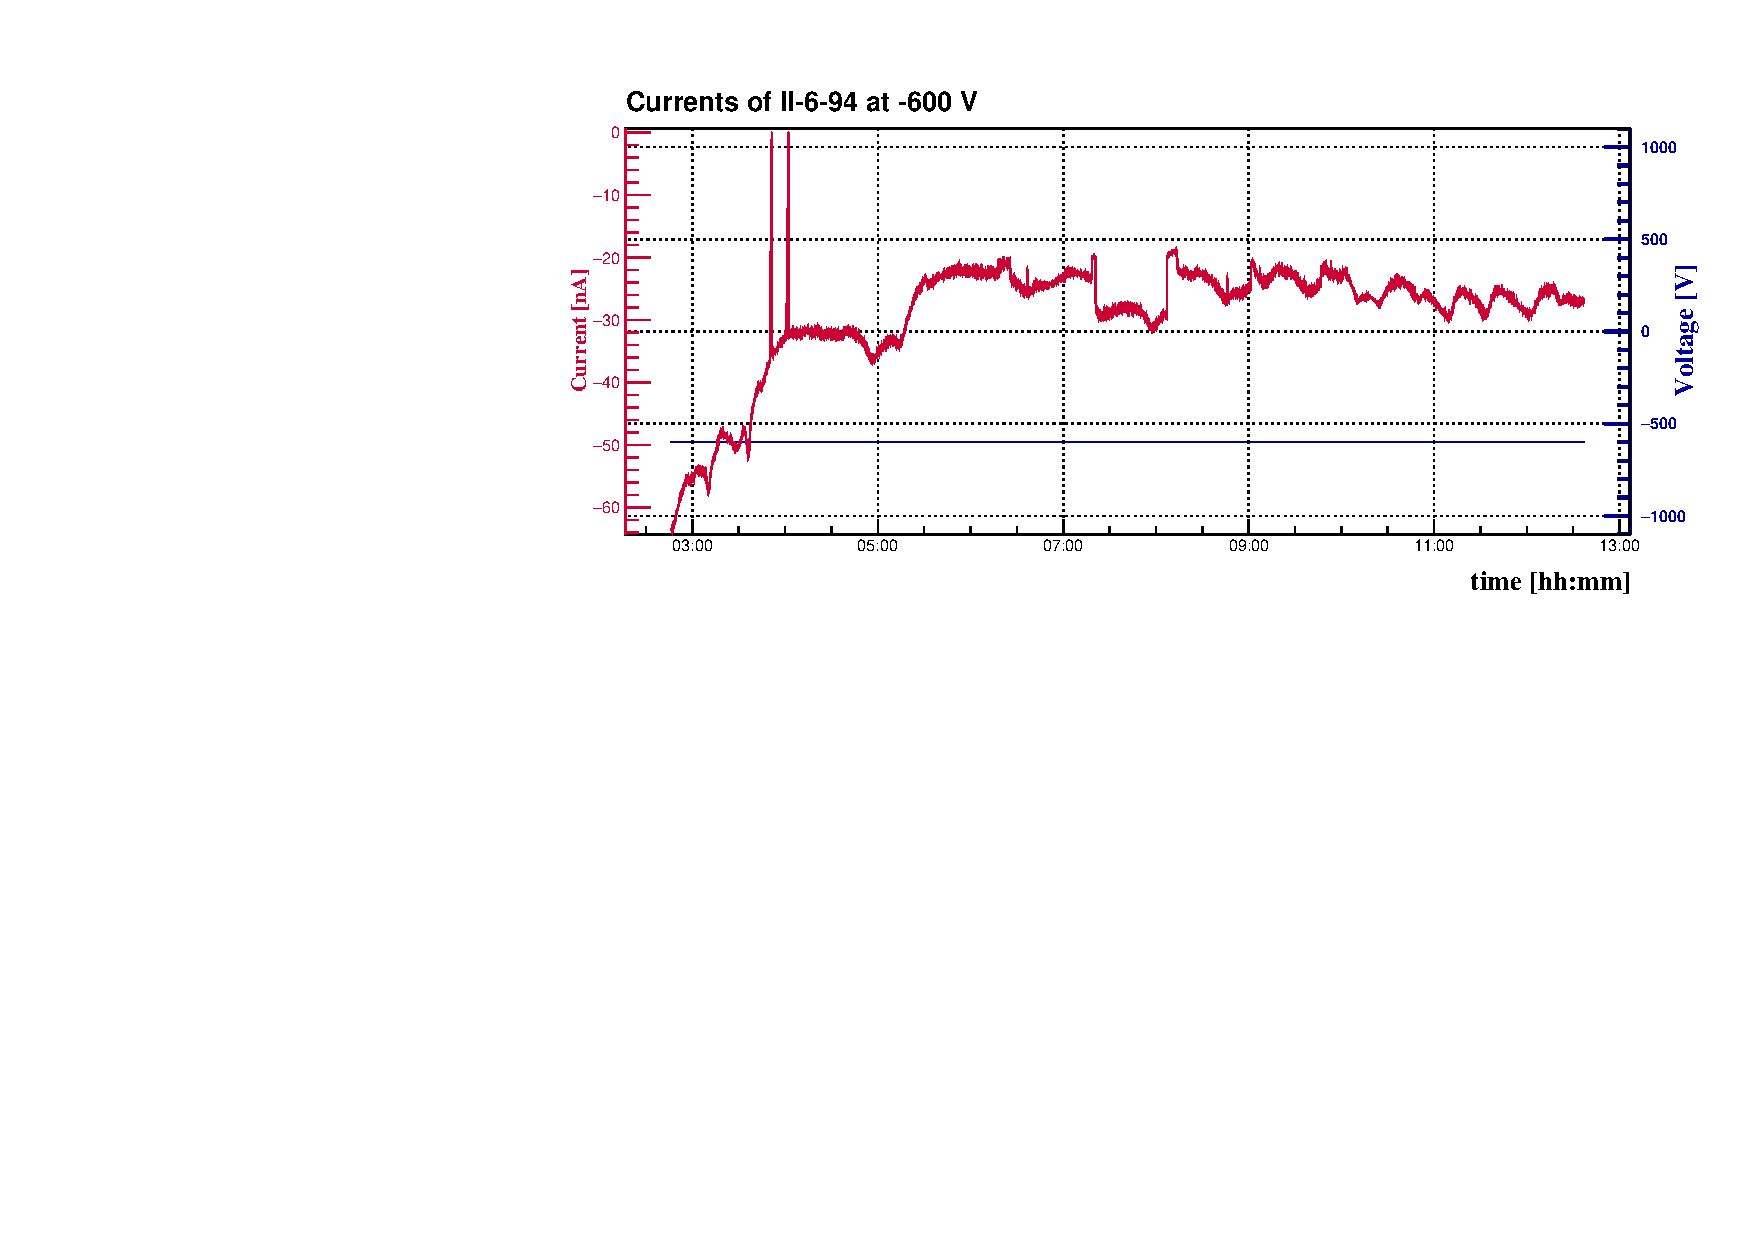
\includegraphics[angle=270, width=11cm]{II-6-94_-600}
	\end{center}
	\begin{itemize}
		\item rather low currents
		\item (almost) no spikes to zero as in Oct 15 beam test
		\begin{itemize}
			\item no beam interruption due to UCN (Ultra Cold Neutrons)
		\end{itemize}
	\end{itemize}
\end{frame}
% ============================
\subsection{$-$\SI{1000}{V}}
\begin{frame}
	\frametitle{$-$\SI{1000}{V}}
	\vspace*{-15pt}
	\begin{center}
		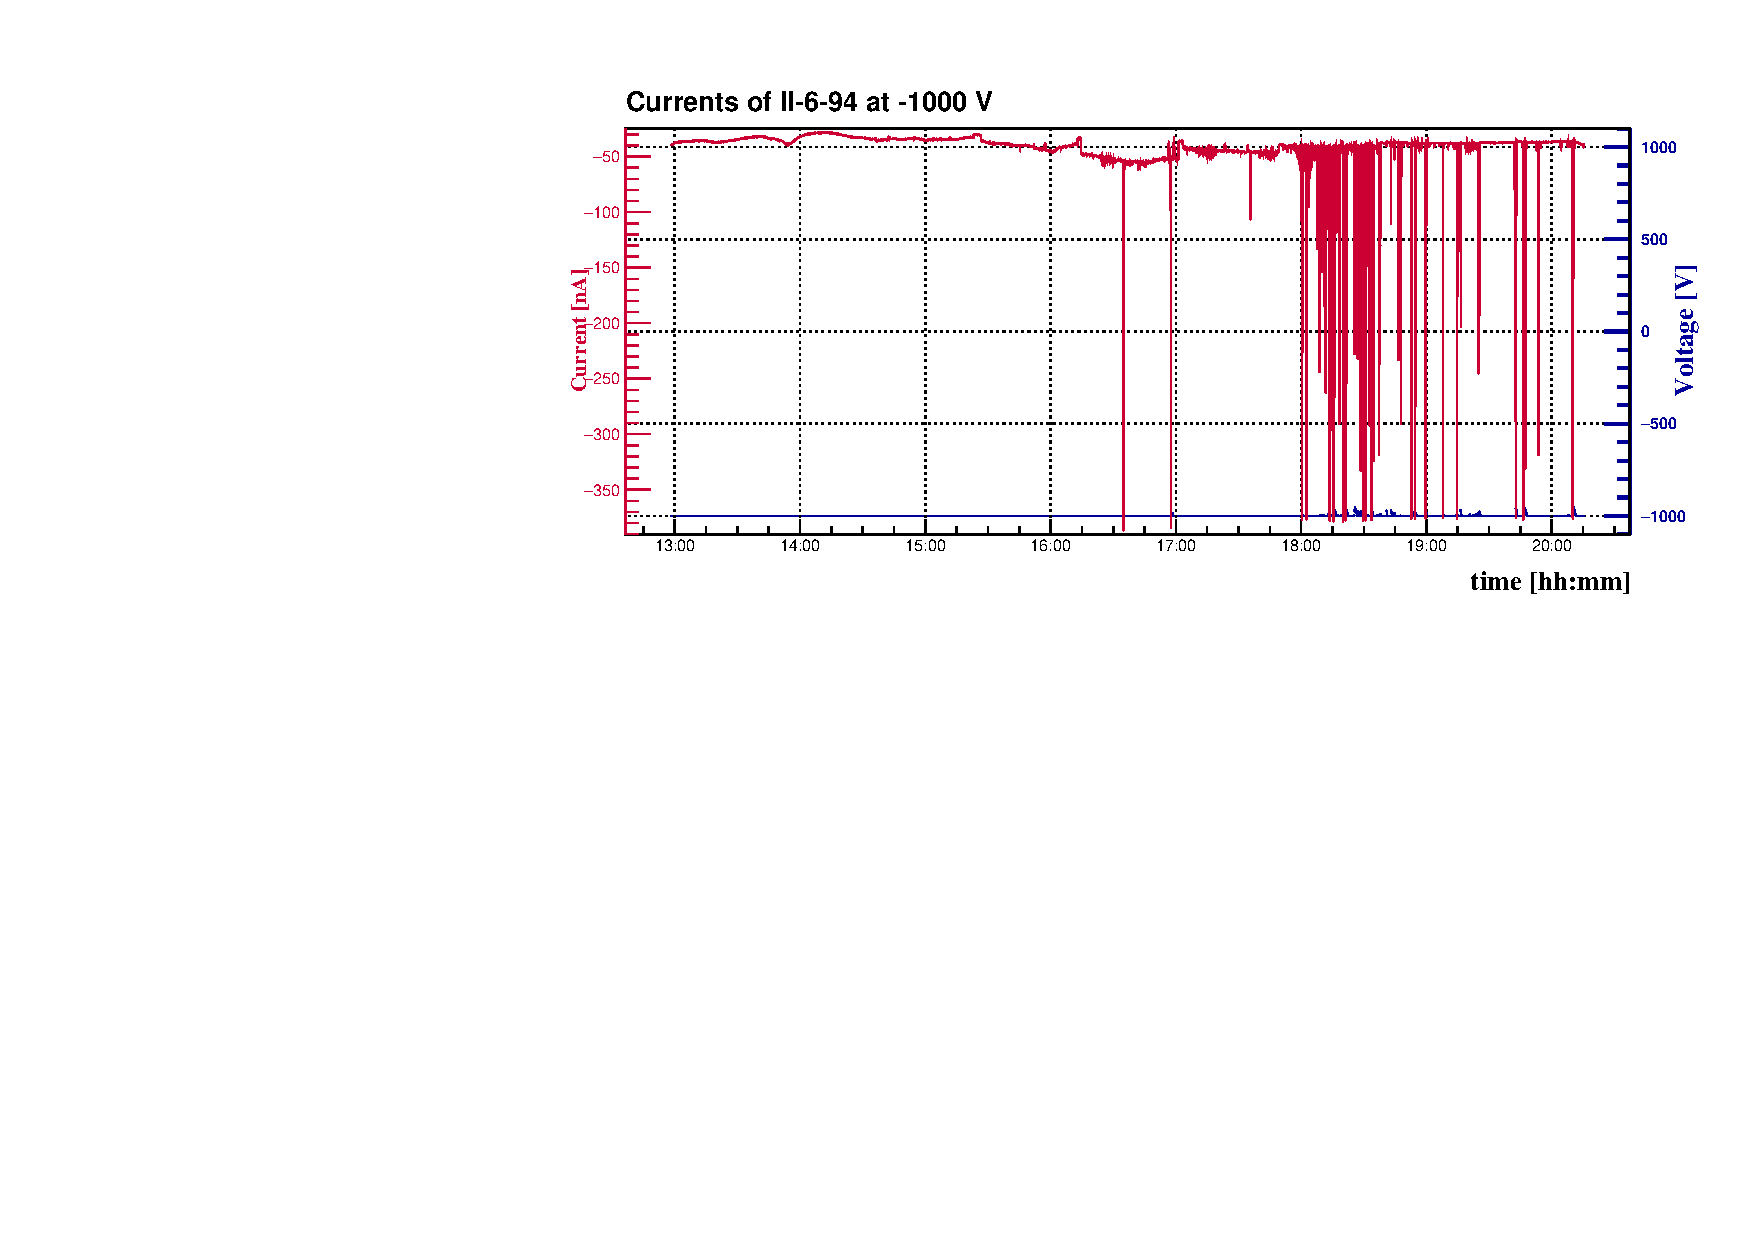
\includegraphics[angle=270, width=11cm]{II-6-94_-1000}
	\end{center}
	\begin{itemize}
		\item current behaviour normal at the beginning
		\item at a certain point in time (high rate) diamond current gets unstable
	\end{itemize}
\end{frame}
% new frame ============================
\begin{frame}
	\frametitle{as Pixel}
	\vspace*{-15pt}
	\begin{center}
		\includegraphics[angle=270, width=11cm]{II6-94_-1000}
	\end{center}
\end{frame}
% END
% ====================================================================================
% BEGIN II6-95
% ====================================================================================
\section{II6-95}
% ============================
\subsection{$-$\SI{1000}{V}}
\begin{frame}
	\frametitle{$-$\SI{1000}{V}}
	\vspace*{-15pt}
	\begin{center}
		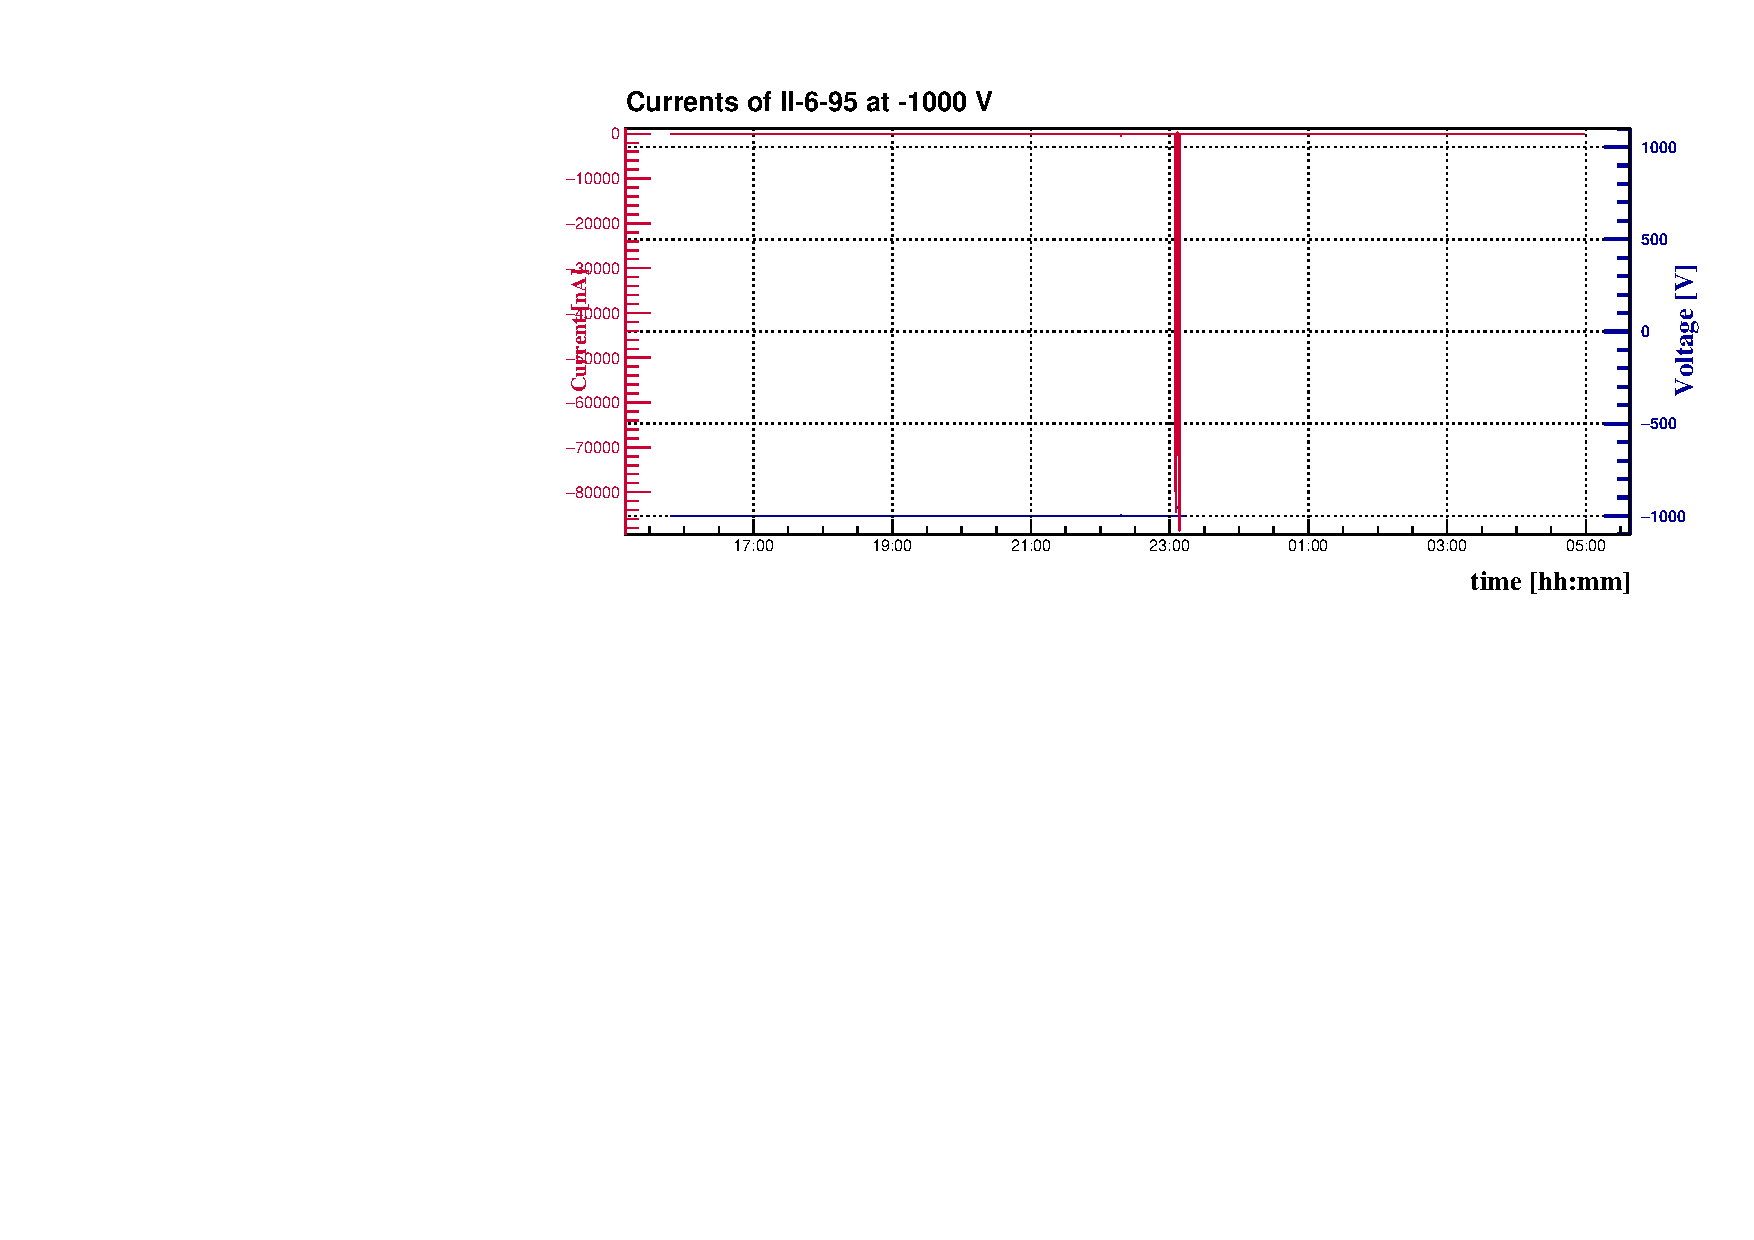
\includegraphics[angle=270, width=11cm]{II-6-95_-1000}
	\end{center}
	\begin{itemize}
		\item 95 installed together with 96
		\item at 11pm one of the Keithleys broke and weird positive currents appeared in both diamonds
		\item change to another Keithley but no monitoring of the current anymore
	\end{itemize}
\end{frame}
% new frame ============================
\begin{frame}
	\frametitle{Zoom}
	\vspace*{-15pt}
	\begin{center}
		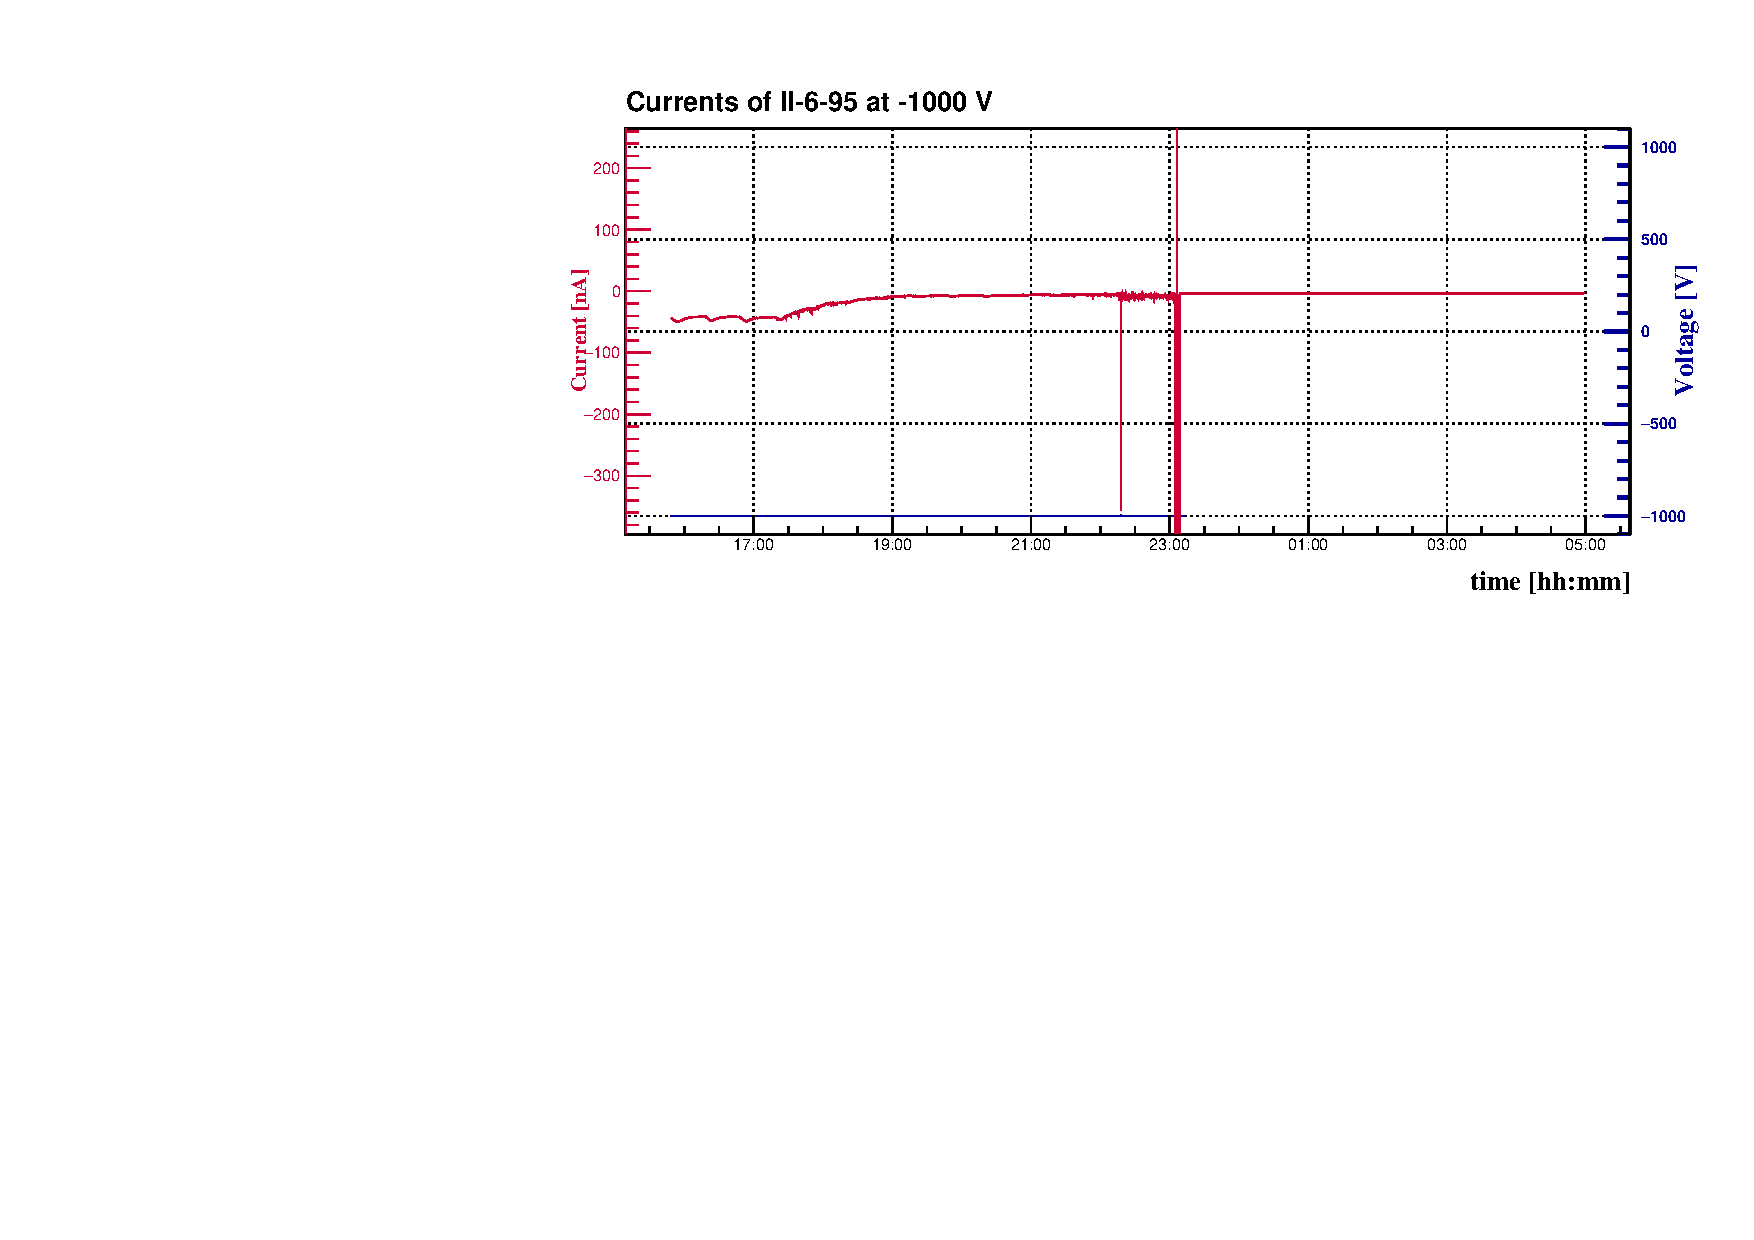
\includegraphics[angle=270, width=11cm]{II-6-95_-1000Zoom}
	\end{center}
\end{frame}
% new frame ============================
\begin{frame}
	\frametitle{as Pixel}
	\vspace*{-15pt}
	\begin{center}
		\includegraphics[angle=270, width=11cm]{II6-95_-1000}
	\end{center}
\end{frame}
% END
% ====================================================================================
% BEGIN II6-96
% ====================================================================================
\section{II6-96}
% ============================
\subsection{$-$\SI{1000}{V}}
\begin{frame}
	\frametitle{$-$\SI{1000}{V}}
	\vspace*{-15pt}
	\begin{center}
		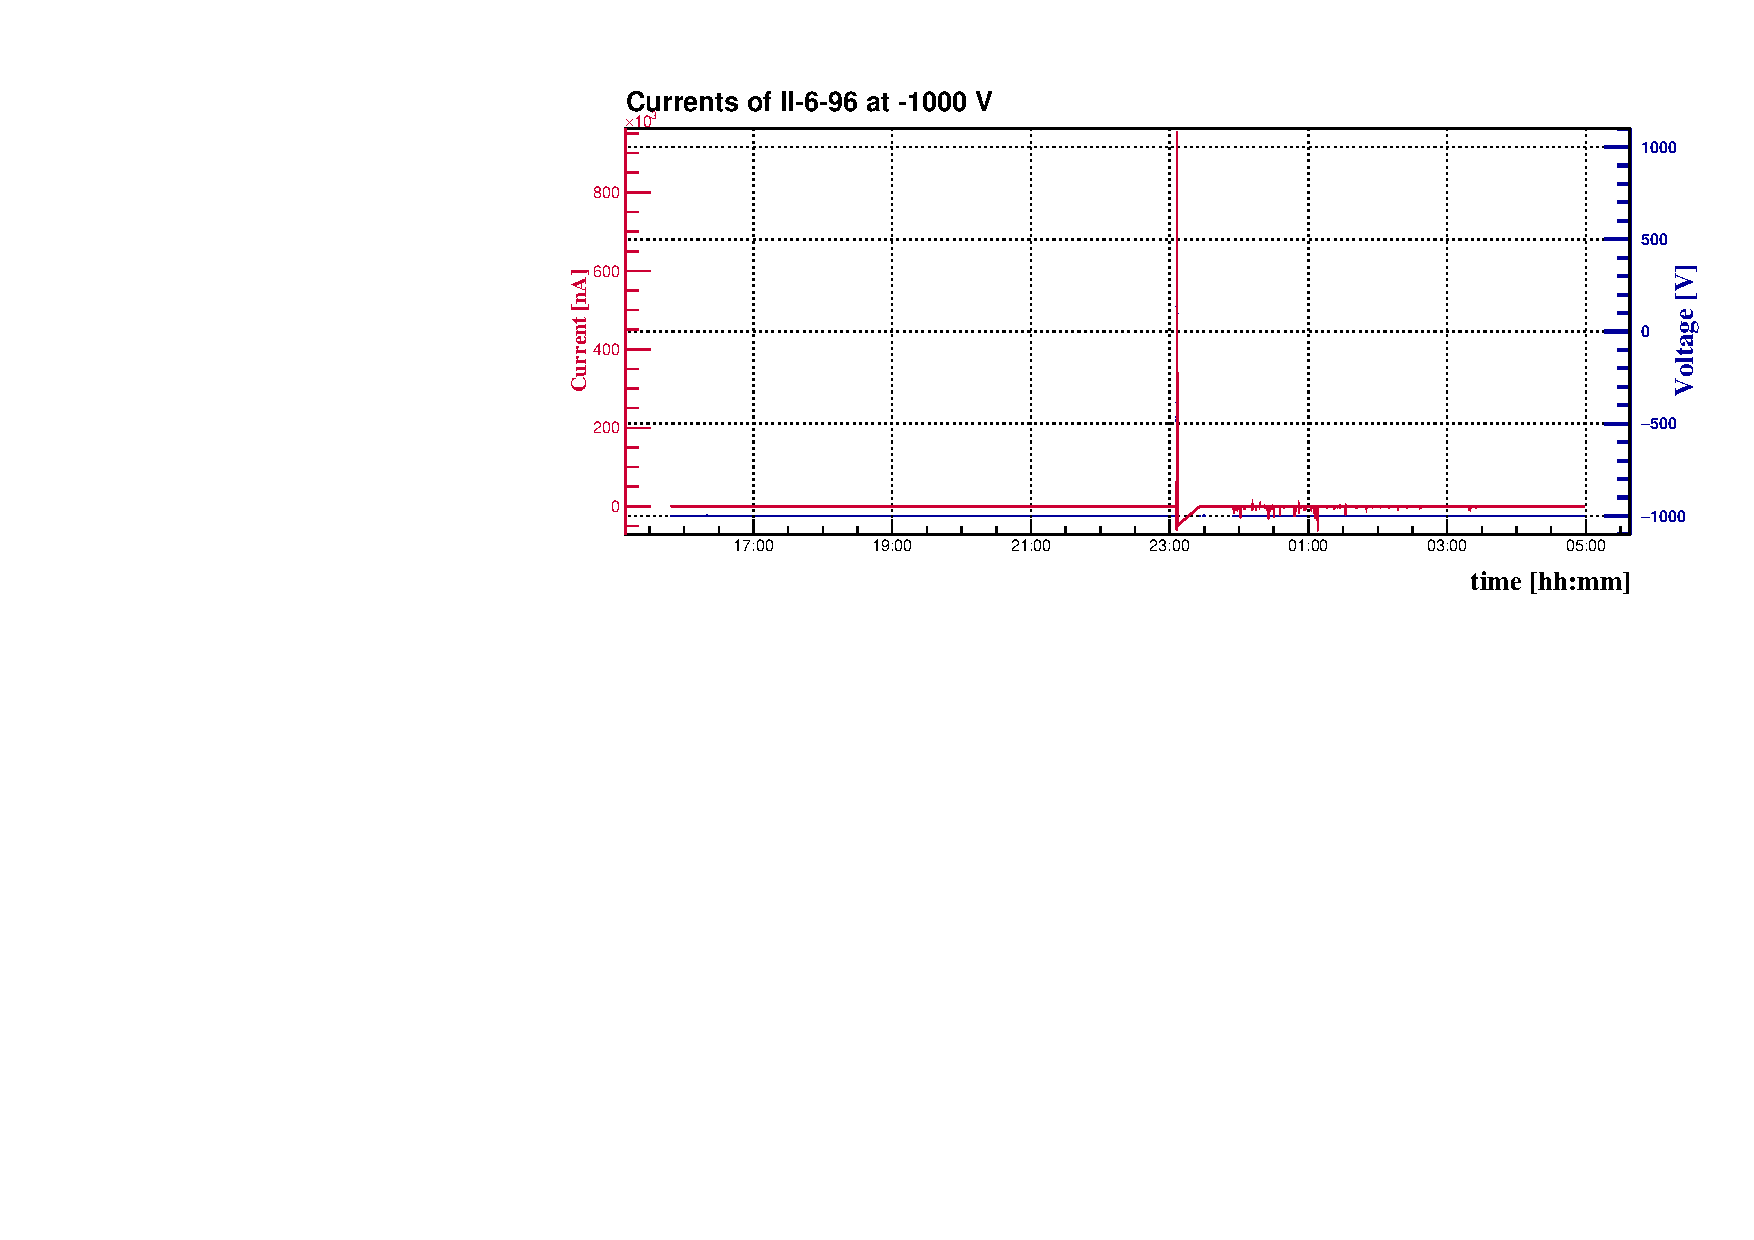
\includegraphics[angle=270, width=11cm]{II-6-96_-1000}
	\end{center}
	\begin{itemize}
		\item very high current spikes after the other Keithley broke
	\end{itemize}
\end{frame}
% new frame ============================
\begin{frame}
	\frametitle{Zoom}
	\vspace*{-15pt}
	\begin{center}
		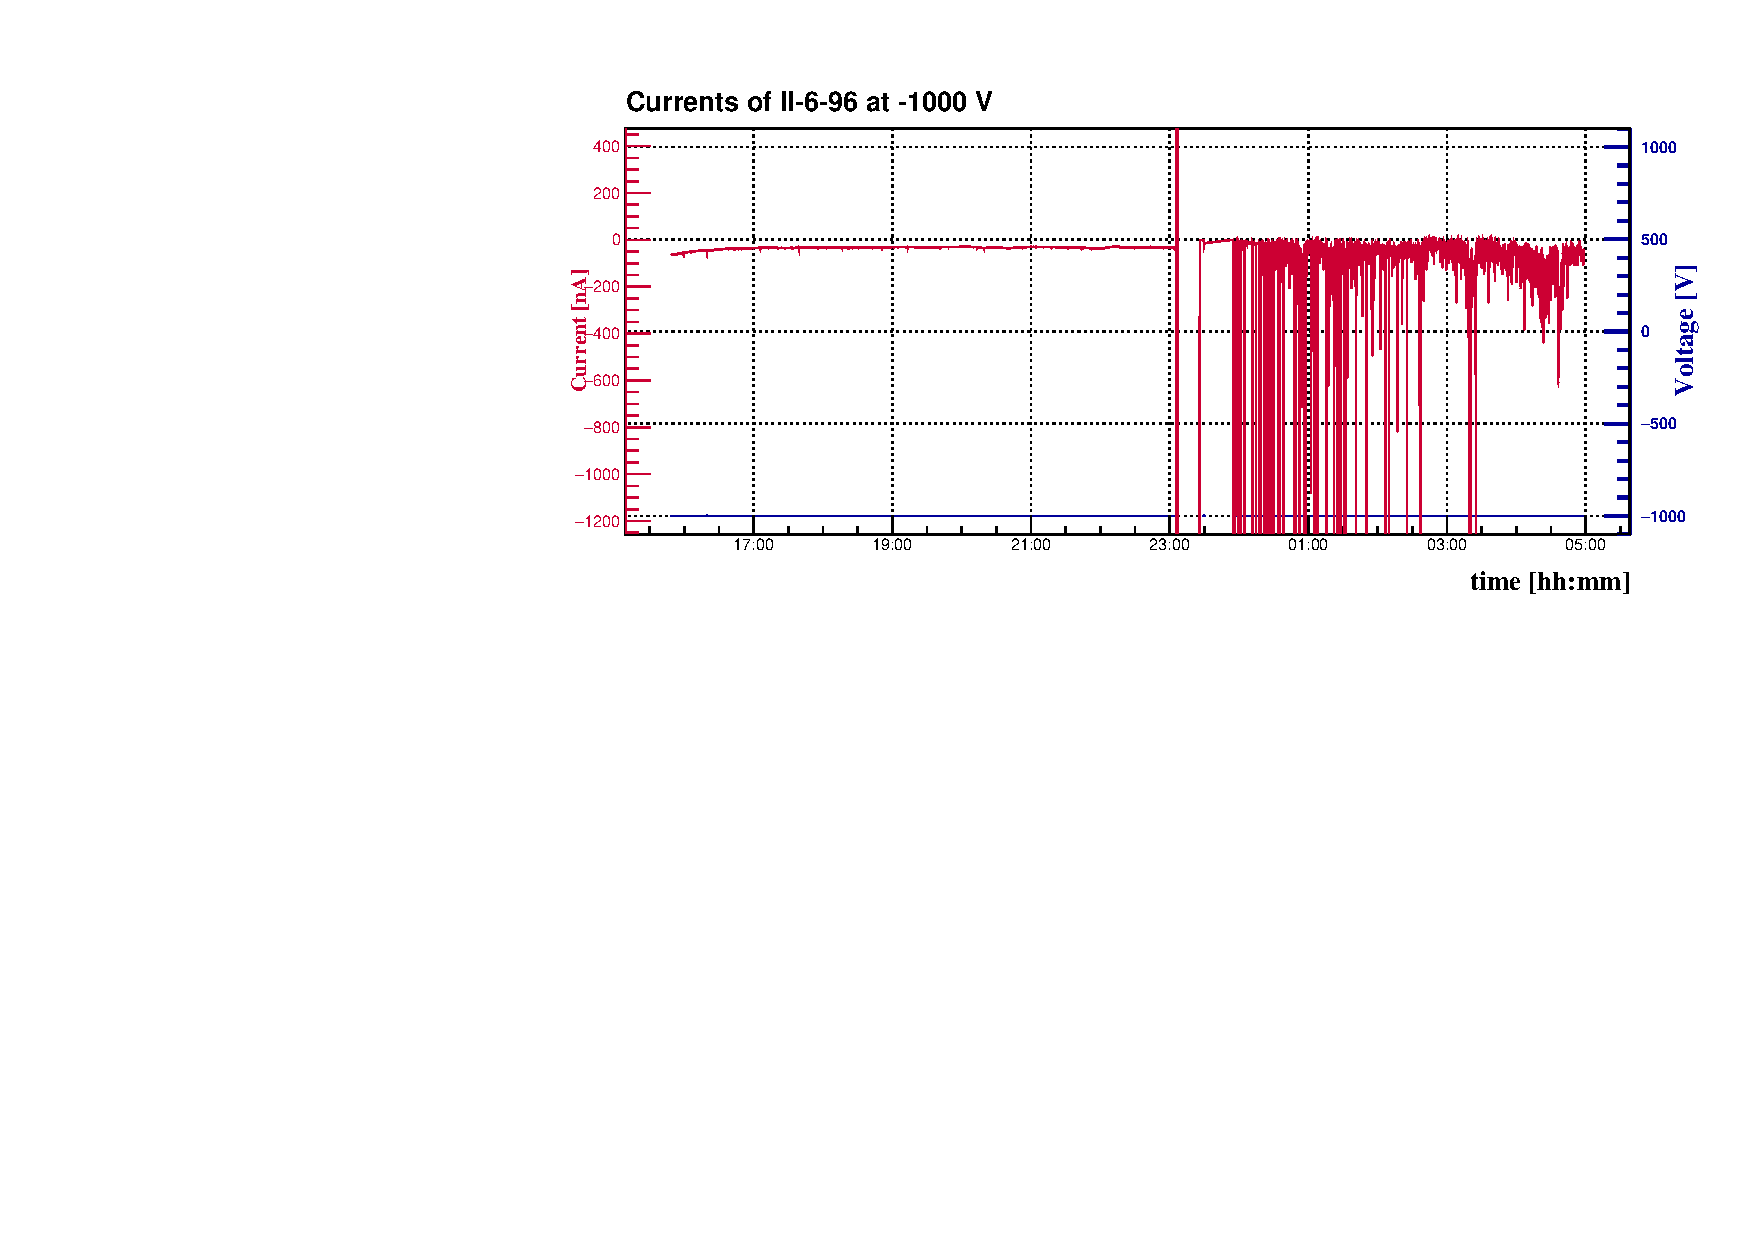
\includegraphics[angle=270, width=11cm]{II-6-96_-1000Zoom}
	\end{center}
\end{frame}
% END
% ====================================================================================
% BEGIN II6-B2
% ====================================================================================
\section{II6-B2}
% ============================
\subsection{$-$\SI{1000}{V}}
\begin{frame}
	\frametitle{$-$\SI{1000}{V} August 2015}
	\vspace*{-15pt}
	\begin{center}
		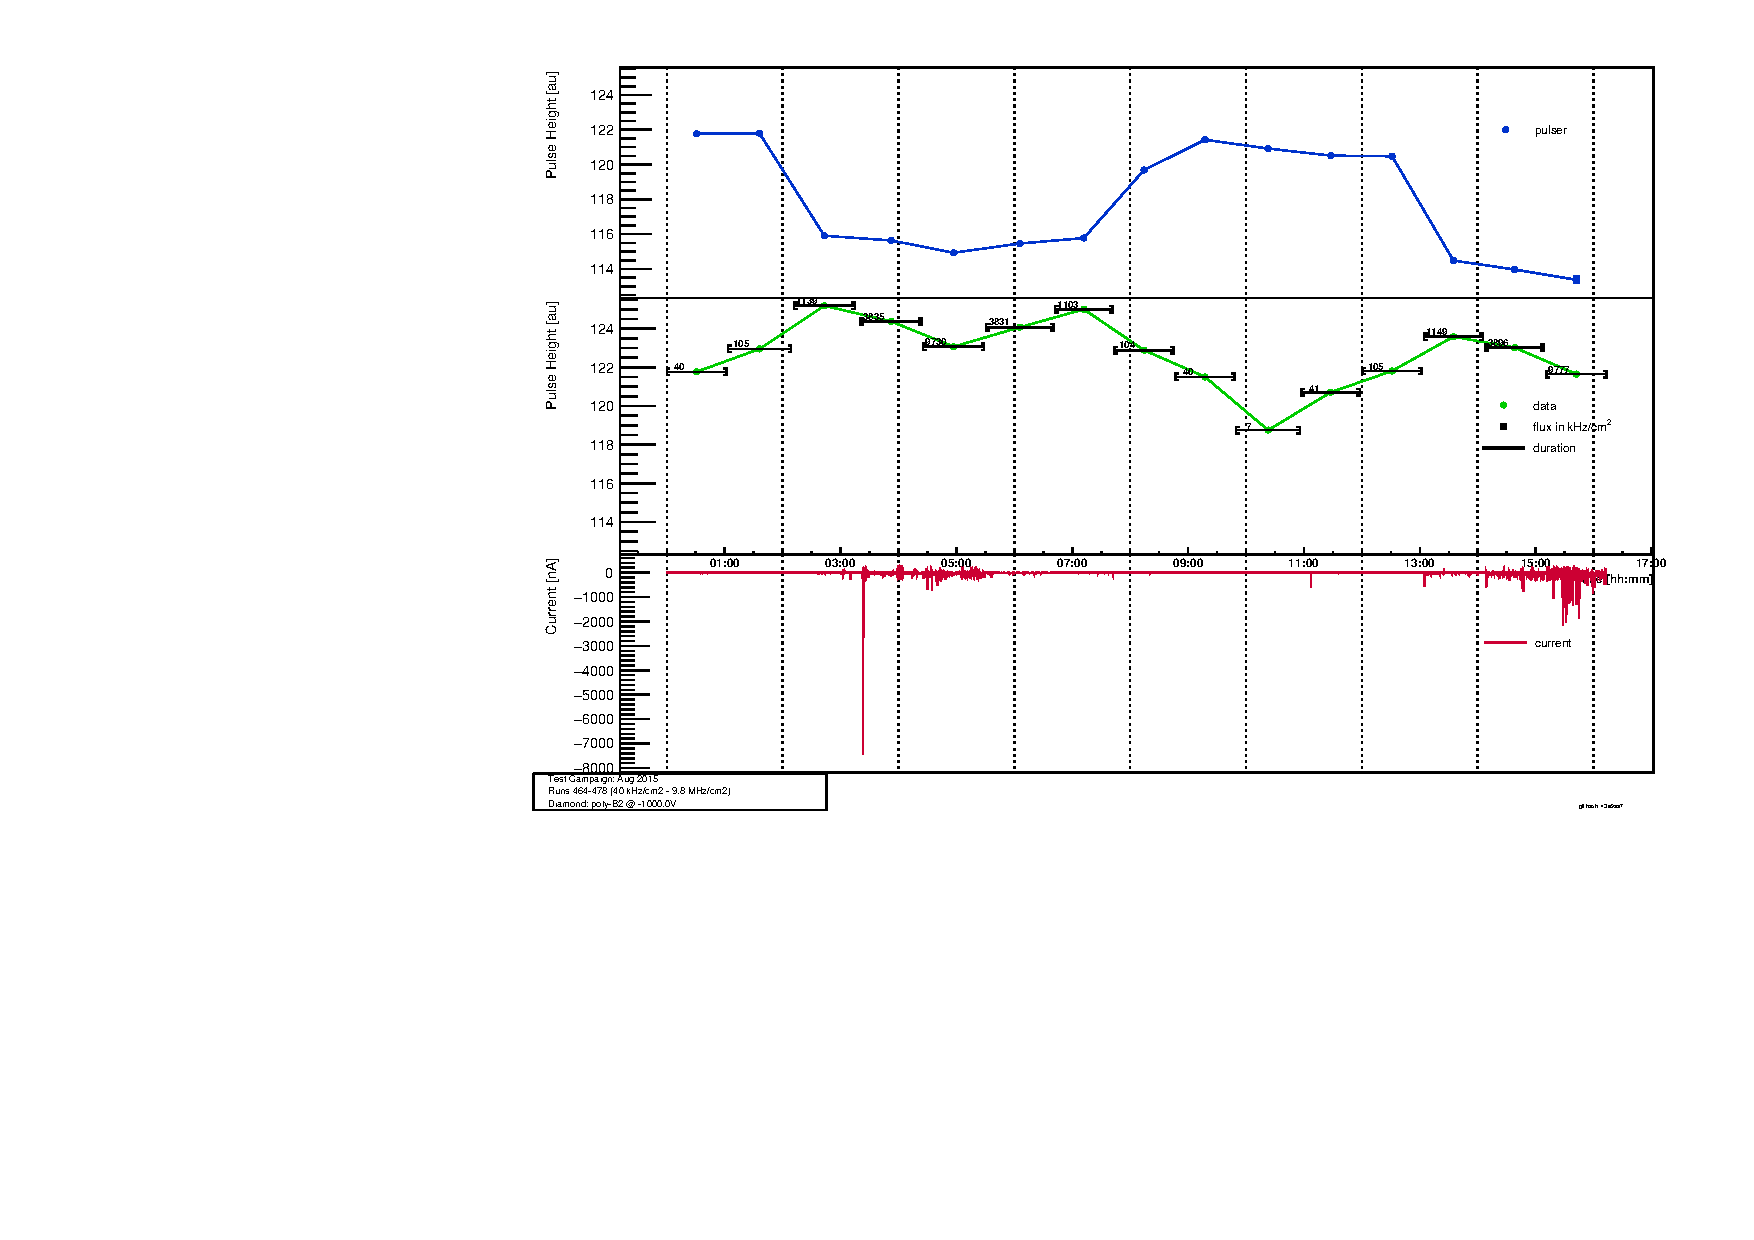
\includegraphics[angle=270, width=11cm]{PhPulserCurrent_201508_rp13B2}
	\end{center}
\end{frame}
% new frame ============================
\begin{frame}
	\frametitle{$-$\SI{1000}{V} October 2015}
	\vspace*{-15pt}
	\begin{center}
		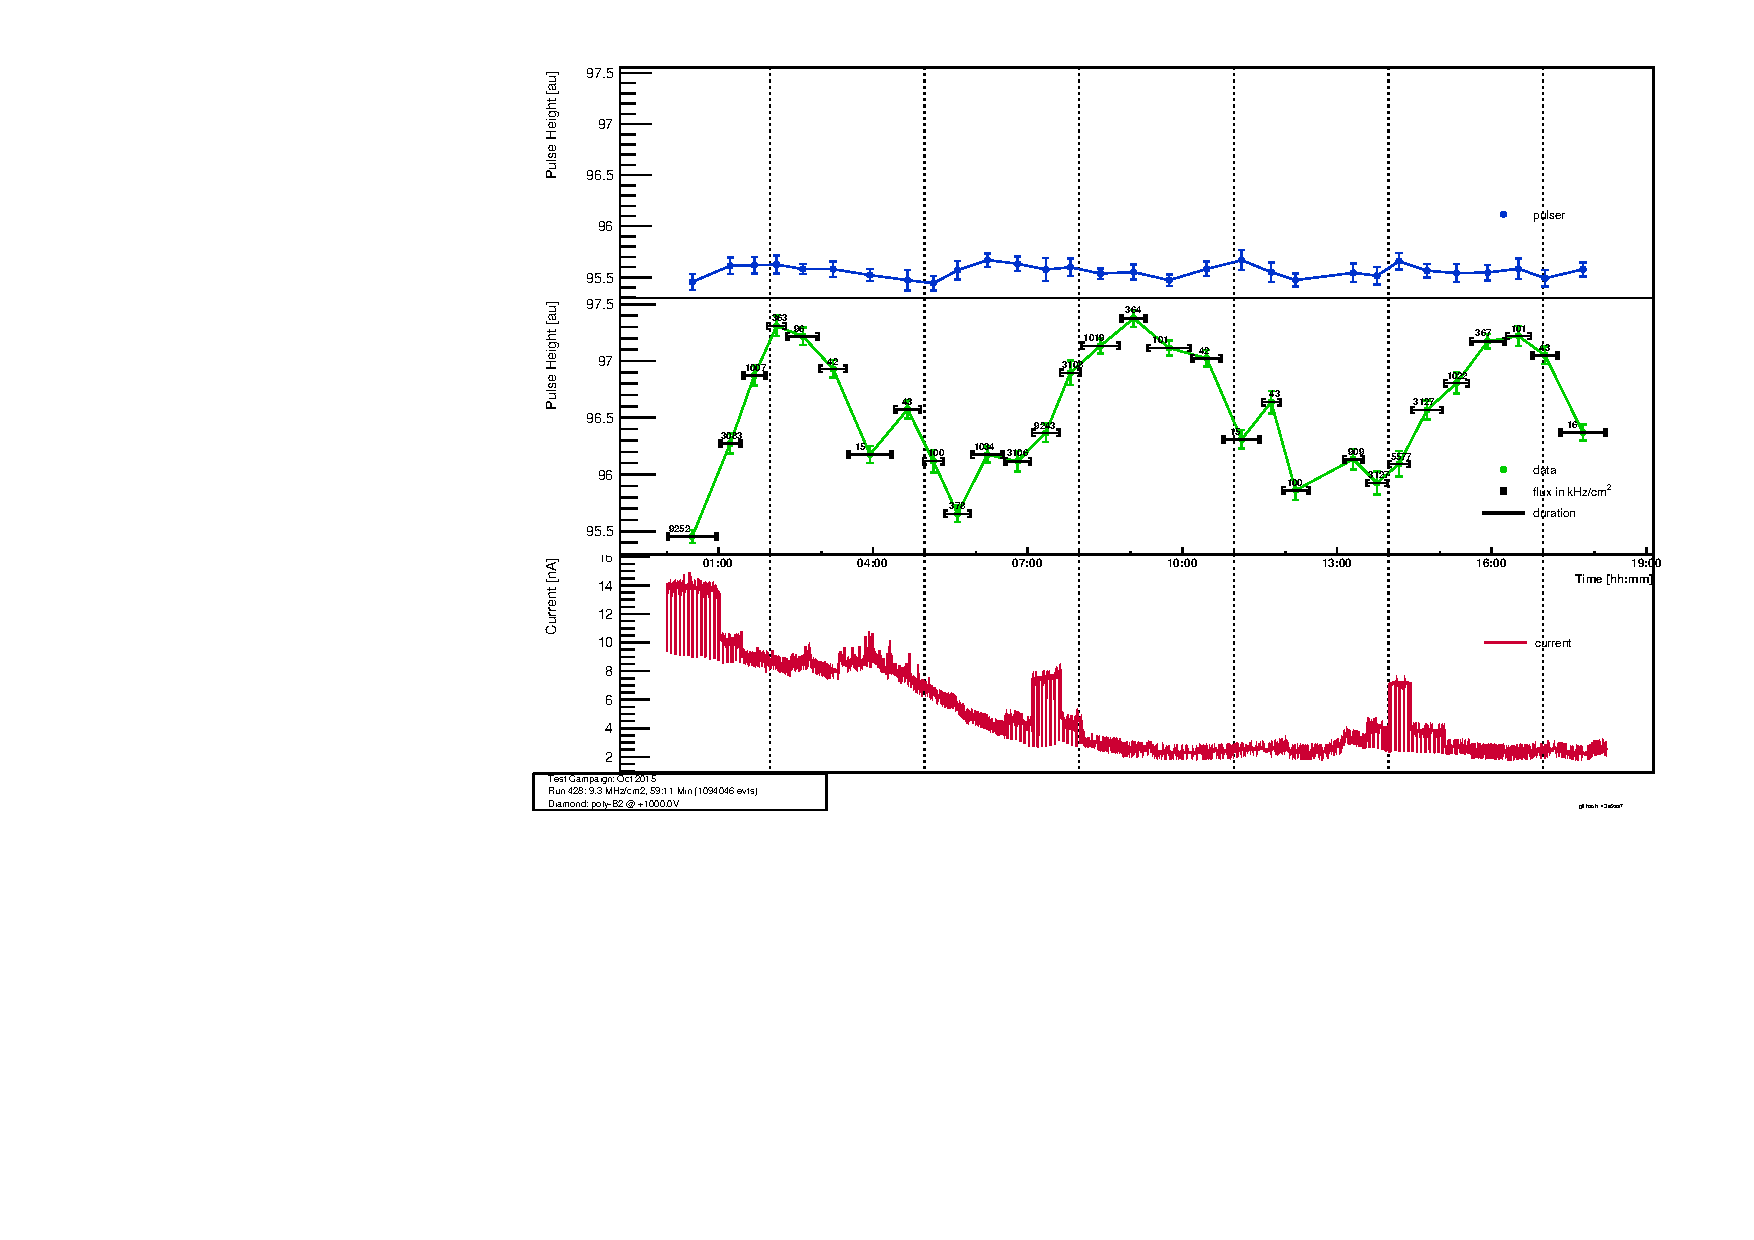
\includegraphics[angle=270, width=11cm]{PhPulserCurrent_201510_rp101B2.pdf}
	\end{center}
\end{frame}
% ============================
\subsection{$+$\SI{1000}{V}}
\begin{frame}
	\frametitle{$+$\SI{1000}{V} October 2015}
	\vspace*{-15pt}
	\begin{center}
		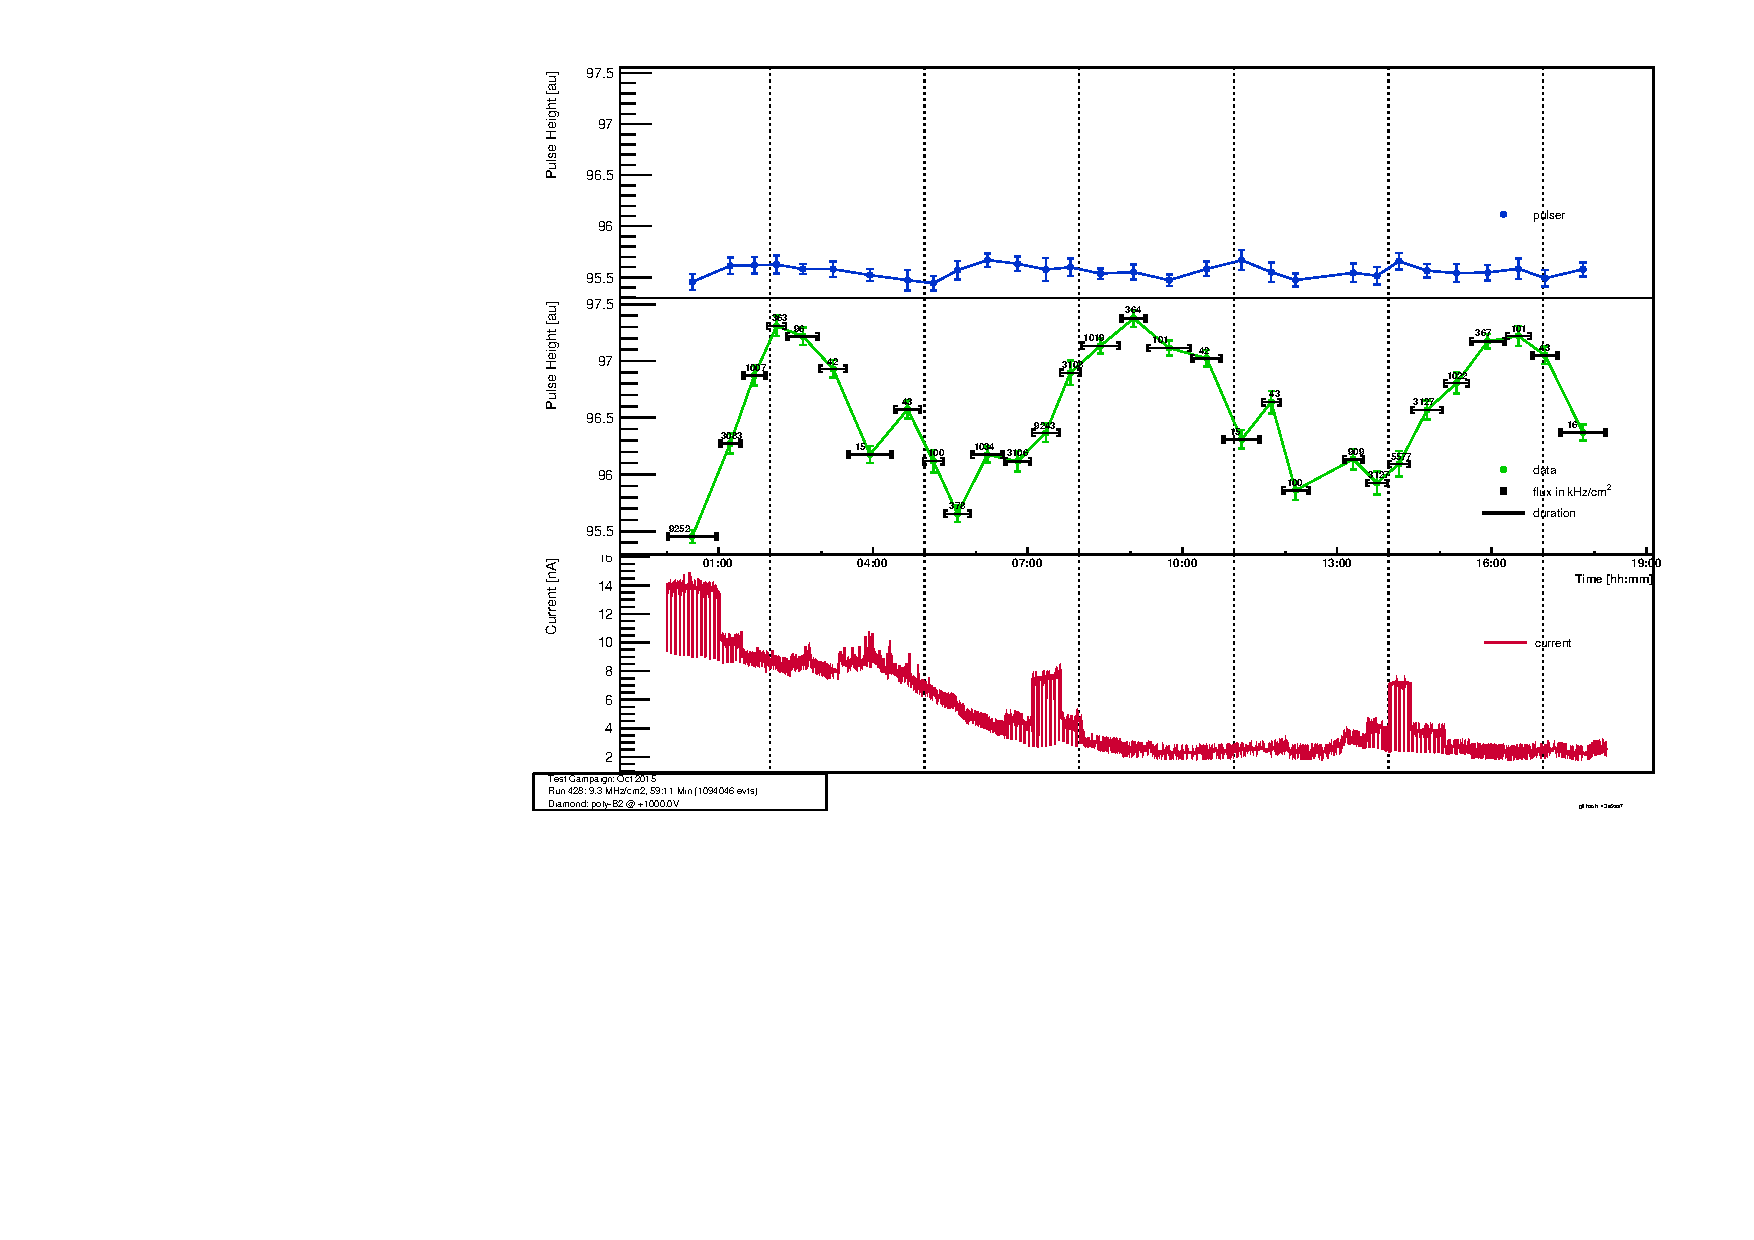
\includegraphics[angle=270, width=11cm]{PhPulserCurrent_201510_rp101B2.pdf}
	\end{center}
\end{frame}
% END
% ====================================================================================
% BEGIN II6-97
% ====================================================================================
\section{II6-97}
% ============================
\subsection{$+$\SI{1000}{V}}
\begin{frame}
	\frametitle{$+$\SI{1000}{V} August 2015}
	\vspace*{-15pt}
	\begin{center}
		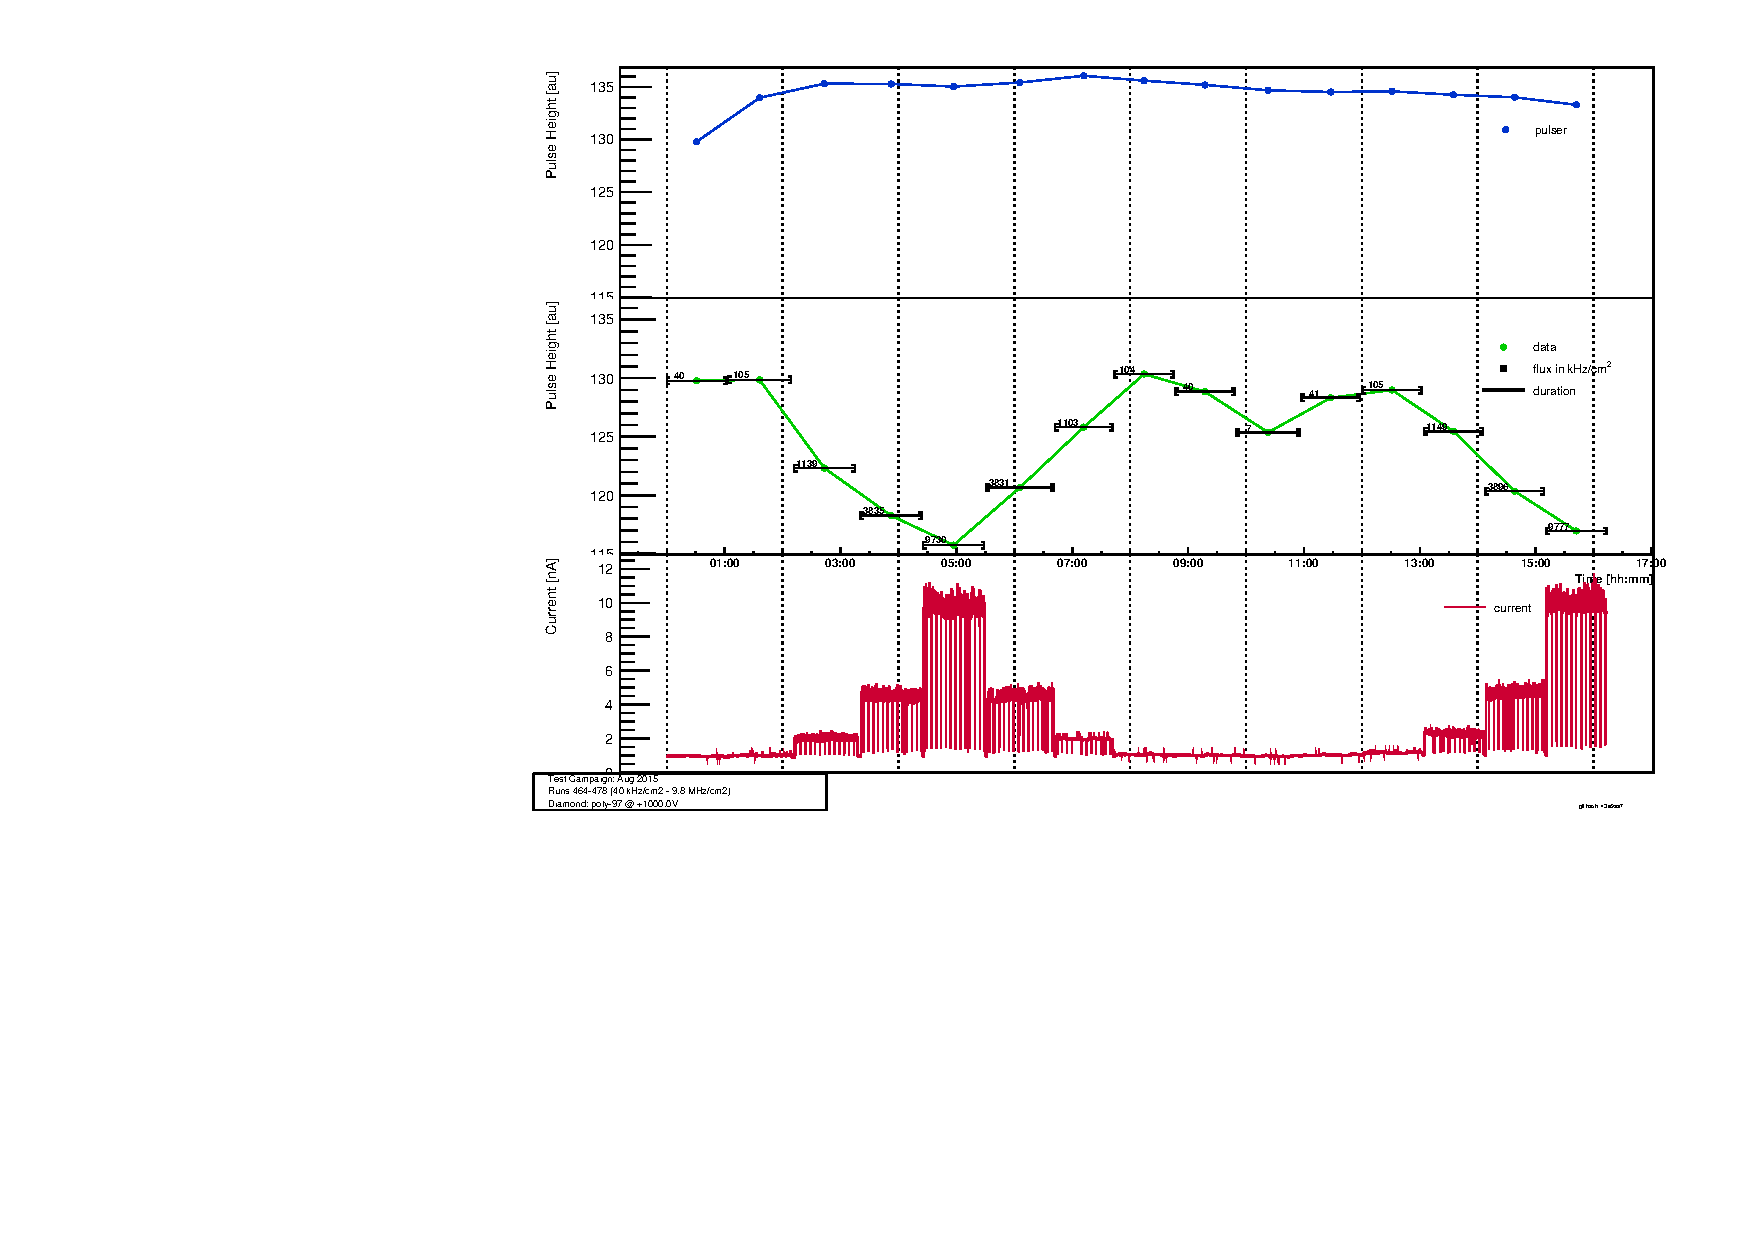
\includegraphics[angle=270, width=11cm]{PhPulserCurrent_201508_rp1397}
	\end{center}
\end{frame}
% ============================
\subsection{$-$\SI{1000}{V}}
\begin{frame}
	\frametitle{$-$\SI{1000}{V} October 2015}
	\vspace*{-15pt}
	\begin{center}
		\includegraphics[angle=270, width=11cm]{II6-97_-1000}
	\end{center}
\end{frame}
% ====================================================================================
% BEGIN CONCLUSION
% ====================================================================================
\section{Conclusion}
% ============================
\begin{frame}
	\begin{minipage}[c][.4\textheight]{\textwidth}
		\begin{itemize}
			\setlength{\itemsep}{\fill}
			\item 94/95/96 show unstabilities at $-$\SI{1000}{V}
			\item 95 stable as pixel at $-$\SI{1000}{V}
			\item 97 and B2 (Oct) stable
		\end{itemize}
	\end{minipage}
\end{frame}
% END
% DOCUMENT END
\end{document}

